\chapter{Introducción}
\label{section:intro}

El presente trabajo tiene como objetivo principal el desarrollo de un sistema de comunicaciones basado en 16-QAM (Modulación de Amplitud en Cuadratura de 16 niveles). Para ello, se propone el empleo en conjunto de los diferentes bloques electrónicos IP estudiados en la asignatura y se divide el desarrollo del entregable en una serie de fases de configuración:

\vspace{2mm}

\begin{itemize}
    \item \textbf{Captura XADC y Memoria FIFO:} En esta primera etapa se realizará la captura de una señal triangular y se procederán a almacenar los datos de entrada en una memoria FIFO.
    \item \textbf{Mapeado QAM: } Se generará el mapeado de 16-QAM para obtener los símbolos a partir de los valores almacenados en la memoria FIFO. 
    \item \textbf{Zero Padding: } Se implementará un upscaling o Zero-Padding con relación 1:32 previo al filtrado para conseguir una respuesta de frecuencia óptima y minimizar la interferencias entre símbolos.
    \item \textbf{Filtrado Root Raised Cosine: } Se deberá generar y aplicar a cada rama I/Q el filtrado pulse shaping del \textit{Root Raised Cosine} (RRC).
    \item \textbf{Mezclador DDS y Multiplicadores: } Se generarán las componentes de transmisión de cada rama I/Q a través de la multiplicación de los valores filtrados por funciones coseno/-seno respectivamente. Estas funciones serán obtenidas a partir de un bloque sintetizador de señal (DDS).
    \item \textbf{Sumador: } Se incluirá un bloque final para la suma de las componentes de transmisión de los caminos I y Q.   
\end{itemize}

\vspace{3mm}

    \begin{figure}[h]
    	\centering
    	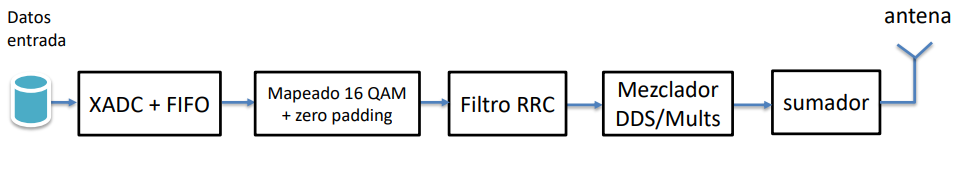
\includegraphics[width=1\textwidth]{img/diseno/sistema.PNG}
    	\caption{Distribución de bloques del sistema de comunicaciones (I)}
    	\label{fig:sistema}
    \end{figure}
    
\vspace{3mm}

Para lograr tanto un correcto funcionamiento de cada bloque electrónico como la interoperabilidad entre ellos al integrarlos en del sistema, será preciso un estudio en profundidad de la documentación proporcionada por el fabricante y un análisis cuantitativo y cualitativo de cada uno de los resultados obtenidos en las simulaciones funcionales. 

    \begin{figure}[h]
    	\centering
    	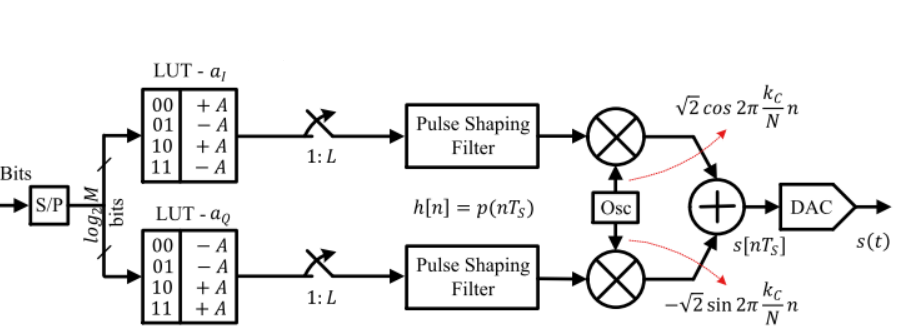
\includegraphics[width=1\textwidth]{img/diseno/sistema2.PNG}
    	\caption{Distribución de bloques del sistema de comunicaciones (II)}
    	\label{fig:sistema2}
    \end{figure}
    
\vspace{3mm}




